\documentclass{article}
\usepackage{ amsmath, amssymb,amsthm}
\usepackage{hyperref}
\usepackage{bm,color}
\usepackage{verbatim}
\usepackage{wrapfig}
\usepackage{caption}
\usepackage{subcaption}
\usepackage{tikz}
\usepackage{tkz-euclide}
\usetkzobj{all}
\usepackage[boxruled,commentsnumbered]{algorithm2e}
\usepackage{booktabs}

\renewcommand{\S}{{\cal S}}
\newcommand{\T}{{\cal T}}
\newcommand{\bigO}{{\bf O}}
%%%%%%%%%%%%%%%%%%%%%%%%%%%%%%%%%%%%%%%%%%%
%%% Environments, Definitions, Commands %%%
%%%%%%%%%%%%%%%%%%%%%%%%%%%%%%%%%%%%%%%%%%%

\newtheorem{definition}{Definition}
\newtheorem{theorem}{Theorem}
\newtheorem{proposition}[definition]{Proposition}
\newtheorem{lemma}{Lemma}
\newtheorem{corollary}[definition]{Corollary}
\newtheorem{observation}[definition]{Observation}
\newtheorem{conjecture}[definition]{Conjecture}
\newtheorem{remark}[definition]{Remark}
\newtheorem{problem}{Problem}
\newtheorem{claim}{Claim}
\newtheorem{open}{Open Problem}
\newtheorem{example}{Example}
%%%%%%%%%%%%%%%%%%%%%%%%%%%%%%%%%%%%%%%%%%%%
%%%%%%%%%%%%%%%%%%%%%%%%%%Hadi's Vars%%%%%%%%%
\newcommand{\points}{\mathcal{A}}
\newcommand{\stepsize}{\gamma}
\newcommand{\Cf}{C_{\hspace{-0.08em}f}}
\newcommand{\y}{\bm{y}}
\newcommand{\z}{\bm{z}}
\newcommand{\s}{\bm{s}}
\newcommand{\shat}{\bm{\hat{s}}}
\newcommand{\bv}{\bm{b}}
\newcommand{\dv}{\bm{d}}
\newcommand{\qv}{\bm{q}}
\newcommand{\uv}{\bm{u}}
\newcommand{\av}{\bm{v}}
\newcommand{\vv}{\bm{v}}
\newcommand{\wv}{\bm{w}}
\newcommand{\xv}{\bm{x}}
\newcommand{\row}{\text{row}}
\newcommand{\col}{\text{col}}
\newcommand{\lft}{\text{left}}
\newcommand{\rgt}{\text{right}}
\newcommand{\dualp}{\bm{\alpha}}
%%%%%%%%%%%%%%%%%%%%%%%%%%%%%%%%%%%%%%%%%%%%%%%

\title{Adapting Training Set Size for  \\ 
Faster Stochastic Gradient Descent Learning}
\author{Hadi Daneshmand, Thomas Hofmann, Aurelien Lucchi}

\newcommand{\w}{{\bf w}}
\newcommand{\x}{{\bf x}}
\newcommand{\risk}{{\cal R}}
\newcommand{\bound}{{\cal H}}
\newcommand{\E}{{\bf E}}
\DeclareMathOperator*{\argmin}{\arg\min}
\DeclareMathOperator*{\argmax}{\arg\max}

\usepackage{hyperref}
 \usepackage{graphicx}
\usepackage{epsfig}
\usepackage{epstopdf}
\graphicspath{ {./images/} }

\begin{document}
\maketitle 

\section{Introduction} 

\paragraph{Large Scale Learning} It is sometimes thought to be a consequence of \cite{bousquet2008tradeoffs} that methods that process a (near-)maximal number of training samples solve the tradeoff between estimation and optimization accuracy in an optimal way. In particular, it is pointed out that SGD needs only $\bigO(1/\epsilon)$ steps to get a generalization error that is $\epsilon$-close to the optimum for strongly convex objectives. As the sampling is i.i.d., the number of distinct samples it will use is
\begin{align}
\tilde n = n \left[1 - \left(\frac{n-1}{n} \right)^t \right]\,.
\end{align}
Note that if $t \ll n \to \infty$, which describes the large scale data regime, $\tilde n \approx t$, as SGD will use a fresh sample in almost every iteration. So without having even visited all data, SGD may already reach a desired accuracy level with regard to the optimal generalization error! 

\paragraph{Stochastic Gradient Descent With Memory} It is a surprising finding that when minimizing additive objectives, composed of $n$ terms, as is the case in (regularized) empirical risk minimization, one can modify SGD to get a much faster, i.e.~linear rate. This happens through memorizing past gradients and by using this information to reduce the variance in the stochastic update directions. The interesting observation for this class of methods is that the rate of the geometric contraction depends inversely on the sample size. The smaller the sample, the faster the rate. Specifically, we get a dependency that takes the form
\begin{align}
\rho_n = 1 - \frac 14 \min \left\{ \frac \mu L, \frac 1 n \right\}
\end{align}
where $\mu/L = \kappa^{-1}$ is the inverse of the condition number. So in the regime, where we have a potentially infinite number of data points, (i) the minimum will be dominated by the (second) $1/n$ term,\footnote{Here we assume that $\mu$ is independent of $n$. As this is somewhat non-trivial for cases, where $\mu$ equals the regularization strength, we will revisit this question later.}  and (ii) the rate will decay in an unfavorable way, $\rho(n) \to 1$ as $n \to \infty$. This  behavior is fundamentally different from that of SGD. We ask the question: how should one resolve the trade-off between estimation and optimization error for this family of variance-reduced SGD methods?

\paragraph{Adaptive Sample Size} The approach we will pursue is to define an effective sample size $n(t) \le N$ that will be used when performing the $t$-th optimization step. The idea is very simple: by reducing the sample size, faster rates are obtained for approaching the corresponding empirical risk minimizer $\w_n^*$ or -- equivalently -- reducing the suboptimality gap relative to the optimum of the $n$-sample risk. At some point however, the optimization accuracy will drop below the statistical accuracy for $n$. Then, by increasing $n$, we can increase the statistical accuracy, at the price of a reduced optimization rate. Ideally, we would increase $m$ in a way that optimally resolves this trade-off in every step. In practice, we will use a mix of \textit{a priori} results as well as data adaptive heuristics  to implement this idea. Throughout upper bounds on the typical quantities (e.g.~expectations with regard to random training samples) control the unknown quantities of interest. 

\section{Adaptive Sample Size Adjustment}

\paragraph{Setting}

We assume that there is some (unknown) distribution $P$ that generates samples $\x \sim P$. For a given sample set $\S = \{\x_i: \x_i \sim P \}$, we denote the empirical risk and its minimizer by 
\begin{align}
\risk_\S(\w) := \frac {1}{|S|} \sum_{\x \in \S} f_\x(\w),
\qquad \w^*_\S := \argmin_\w \risk_\S(\w) 
\end{align} 
Moreover, we define the expected risk of a solution as $\risk(\w) := \E f_\x(\w)$ and its minimum and minimzer by $\risk^*$ and $\w^*$, respectively. 

\paragraph{Generalization Bounds}

Generalization bounds aim at uniformly bounding the deviation between the empirical and the expected risk over the function class at hand. A typical bound takes the form
\begin{align}
\E_\S \left[ \sup_{\w} \left| \risk(\w) - \risk_\S(\w) \right| \right]  \leq
\bound(n) \label{eq:bound}
\end{align} 
where the expectation is over a random sample $\S$ of fixed size $|\S|=n$. Here $\bound$ is a bound that depends on $n$, usually in a ratio $n/d$ relative to some capacity measure $d$ of the function class (e.g.~in the linear case the dimensionality or the VC dimension), which we assume to be constant in our discussion.  A simple, often conservative bound may scale as $\bound(n) \in \bigO(1/\sqrt{n})$. It is sometimes possible to derive more optimistic bounds on the estimation accuracy (e.g.~in the realizable case) such as $\bound(n) \in \bigO(\log(n)/n)$ or even $\bound(n) \in\bigO(1/n)$.  We favor, of course, thighter bounds, but which bound to apply is problem-specific.

Note that the bounds hold with high probability over the choice of the sample set. So there could always be sample sets that violate the bound. Morever, the uniform convergence (supremum over all solutions $\w$) is required to allow dependencies between $\w$  and the (random) data. It holds in particular it holds for $\w$ that are minimizer of empirical risks or approximations thereof. 

\paragraph{Bounds on Suboptimality} 

Assume we have some solution $\w_\S$ that is (by design) guranteed to be an $\epsilon$-approximation in the empirical risk, namely $\risk_\S(\w_\S) - \risk_\S^* \le \epsilon$.  We can bound its $P$-suboptimality in expectation over the random choice of $\S$ as follows 
\begin{align}
\label{eq:exprisk-bound}
\E \risk(\w_\S) - \risk^*  & = 
\E \left[ \risk(\w_\S) \mp \risk_\S(\w_\S) \mp \risk_\S(\w_\S^*) \mp \risk_\S(\w^*) \right]   - \risk(\w^*)
% \\  & \le \E \sup_\w \{ | \risk(\w) -  \risk_\S(\w) | \} + \epsilon + 0 + \E \risk_\S(\w^*) - \risk(\w^*) 
\\ & \le \E \sup_\w \{ | \risk(\w) -  \risk_\S(\w) | \} + \epsilon  \le  \bound(n) + \epsilon 
\nonumber
\end{align}
This mean, we can basically add up bounds on the statistical accuracy and the optimization error. 



\paragraph{General Idea}

We assume that our iterative optimization method can reduce the optimization error and thus by the above result the $P$-suboptimality  
\begin{align}
\epsilon_\S^t =   \epsilon \rho_n^t  \quad (\rho_n <1), \quad  
\text{i.e.} \quad 
\E \risk(\w^{\S+t}_\S) - \risk^*  \le \bound(n) + \epsilon\rho_n^t 
\end{align}
Obviously, even as $t \to \infty$, we can never improve on the statistical accuracy. We want to know, how much could be gained by increasing the sample size to $N$ and by sampling $\delta n := N - n$ additional data points from $P$. Of course, we can use the same bound by replacing $n$ with $N$. The only question is how we can control the optimization accuracy on the extended sample $\T \supset \S$. 

\paragraph{Optimization Error on Enlarged Sample}
We consider the chain:
\begin{align}
\risk_\T(\w_\S) - \risk_\T^* = \risk_\T(\w_\S) \stackrel{[1]}{\mp} \risk_\S(\w_S) \stackrel{[2]}{\mp} \risk_\S(\w_\S^*) \stackrel{[3]}{-} \risk_\T(\w_\T^*)
\end{align}
We bound the three involved differences as follows: 
\begin{align}
\text{[2]} \quad & \risk_\S(\w_S)  - \risk_\S(\w_\S^*) \le \epsilon  \qquad 
\text{($\epsilon$ optimality of $\w_\S$ with regard to $\risk_\S$)}
\\
\text{[3]} \quad & \E_\T \left[ \risk_\S(\w_\S^*) - \risk_\T(\w_\T^*) \right] \le 0 \qquad 
\text{(optimizing over a subsample)}
% \\
%& \E_\T \left[ \risk_\S(\w_\S^*) - \E_{\T} \risk_\T(\w_\S^*) \right] \le 0 \qquad 
%\text{(since $\E\risk_\S(\w^*_\S) \le \risk(\w_\S)$)}
\end{align}
The latter inequality can be justifed by
\begin{align}
\E_{\S} \risk_\S(\w_\S^*) \stackrel{[4]}{\le} \E_{\T} \risk_\S(\w_\T^*)  \stackrel{[5]}= \E_{\T} \risk_\T(\w_\T^*)  
\end{align}
where 
\begin{align}
\text{[4]} \quad & \risk_\S(\w_\S^*) \le \risk_\S(\w), \quad \forall \w\\
\text{[5]} \quad & \E_{\S | \T} \risk_\S(\w) = \risk_\T(\w), \quad \forall \w \quad \text{as $\S \subset \T$}
\end{align}
Moreover, we have that
\begin{align}
& \E_{\T-\S} \left[ \risk_\T(\w_\S) - \risk_\S(\w_S) \right] \le \frac{N- n}{N} | \risk(\w_S) - \risk_\S(\w_\S) |
\label{eq:t-s} \qquad 
\end{align}
and hence 
\begin{align}
\text{[1]} \quad & \E_{\T} \left[ \risk_\T(\w_\S) - \risk_\S(\w_S) \right] \le \frac{N-n}{N} \sup_\w | \risk(\w) - \risk_\S(\w) | \le \frac{N-n}{N} \bound(n)
\label{eq:t-s-all} 
\end{align}
%
So we finally arrive  at 
\begin{align}
\E \left[ \risk_\T(\w_\S) - \risk_\T^*\right] \le \epsilon + \frac{N-n}{N} \bound(n)
\label{eq:new-epsilon} 
\end{align}

Let us sanity-check this. We have two generalization bounds 
\begin{align}
\epsilon + \bound(n) 
\stackrel{?}{\le}
\epsilon + \frac{N-n}{N} \bound(n) + \bound(N)  
\iff \frac nN \bound(n) \le \bound(N)
\end{align}
So for $\bound(n) = c/n$ we get 
\begin{align}
\frac nN  \frac{c}{n} = \frac cN \leq \frac cN \quad \text{(ok)}
\end{align}
and for $\bound(n) = c/\sqrt{n}$ we get  
\begin{align}
\frac nN  \frac{c}{\sqrt n}  = \frac{n}{\sqrt{N} \sqrt{n}}  \frac{c}{ \sqrt N} < \frac c {\sqrt{N}} \quad (ok)
\end{align}

\paragraph{Sample Size Adaptation}

The challenge is that whenever we switch to a larger sample size, we may have some additional slack that comes from the application of further bounds such as on the right-hand side of \eqref{eq:new-epsilon}, which is likely to overestimate the optimization error. So if we just look ahead of how the bounds evolve for a single iteration, we will never switch (this can be seen by comparing the increase in $\epsilon$ with what we gain in terms of statistical accuracy). However, we can overcome this issue by specifying a horizon $T$, i.e.~the number of iterations that we plan to perform in total. Then the conservativism in the bounds will be amortized over many iterations. 

The optimal sample size schedule  can be obtained by dynamic programming. 
\begin{align}
U(t,n,\epsilon)  
& = \min \left\{ U \left(t-1,n, \epsilon \rho_n \right),  \min_{\delta n \ge 1} U_{\delta n}(t,n,\epsilon) \right\} 
\label{eq:recursion_first}\\
U_{\delta n}(t,n,\epsilon)  
& :=  U \left(t, n + \delta n, \epsilon  + \frac{\delta n}{n+\delta n} \bound(n) \right) \\
U(0,n,\epsilon) &= \epsilon + \bound(n)
\end{align}
Here the grounding is at the point where no further iterations are left. Note that $n \le T$. The first minmum compares the case, where we continue with the same sample size vs.~increasing. The second (nested) minumum picks the optimal increment for the sample set increase.  

%\newpage
%[OLD STUFF]
%\newpage
%
% Hadi's ==========================
\begin{remark}
 Consider we are iterating on $n$ samples and we want to figure out when is the
 best time to switch from $n$ to $n+\Delta n$. This problem is a step back from
 our recursive formulation. Still, it is useful to simplify the switching
 condition. We iterate on $n$ samples as long as: 
 \begin{equation*}
		\epsilon \rho_n^t + \bound(n) \leq \left\{ \rho_{n+\Delta
		n}\left( \epsilon \rho_{n}^{t-1} + \frac{\Delta n}{ n + \Delta n} \bound(n)  
		\right)+\bound(n + \Delta n) \right\} 
	\end{equation*}
Assume we use SAGA, i.e. $\rho_n = 1-1/n$, and $\bound(n) = 1/n$, then we can
proceed to simplify above formulation. 
\begin{eqnarray*}
		& \epsilon \rho_n^t + \bound(n) - \left\{ \rho_{n+\Delta
		n}\left( \epsilon \rho_{n}^{t-1} + \frac{\Delta n}{ n + \Delta n} \bound(n)  
		\right)+\bound(n + \Delta n) \right\} \\ 
		& = \epsilon \rho_n^{t-1} (\rho_n - \rho_{n+\Delta n}) +\bound(n)
		-\bound(n+\Delta n) -\rho_{n + \Delta n	} \left( \bound(n) - \bound(n+ \Delta
		n) \right) \\ 
		& = \bigg[1 -\epsilon \rho_n^{t-1} -\rho_{n+\Delta n}\bigg]\left( \bound(n) -
		\bound(n + \Delta n) \right) \\ 
		& = \bigg[\bound(n+\Delta n) - \epsilon \rho_n^{t-1}\bigg] \bigg[ \bound(n) -
		\bound(n + \Delta n)\bigg]
	\end{eqnarray*} 
We know that $\bound(n) \geq \bound(n + \Delta n)$ always holds, therefore we
iterate on $n$ as long as sub-optimality on $n$ samples is larger than
statistical efficiency of sample size $n + \Delta n$, i.e. $\bound(n + \Delta n)
\leq \epsilon \rho_n^{t-1}$.
\end{remark}
\textbf{ The main drawback of the recursion equation \ref{eq:recursion_first}:}
As we mentioned in appendix, for different optimization error $\epsilon$ we can
choose the different increase in sample size i.e. $\delta n$. So, $\delta n$ is a
function of $\epsilon$. Consequently, we have to minimize the recursion equation
respect to $\epsilon$. The $\epsilon$ itself depends on the number of
iterations $t$. In addition, the $\epsilon$ is continues and this makes 
problem with dynamic programming, which usually involves discrete variables.
We aimed to remove the challenging $\epsilon$ in the next step. 
\paragraph{New scheduling for the sample size:}
For slow convergence rate, as Thomas mentioned, the
recursion formula chooses the small sample size to iterate on and never switches to the larger sample size.
Indeed, we need new dynamic programming to include the time horizon $T$ in our analysis. Consider we are limited to $t$
iterations on sample size $n$. We can split our budget, which is the number of
iterations $t$, to two parts: spare $\alpha$ iteration for $n$ samples, $t-\alpha$ iterations on a sub-sample with size $n-\beta$. In this case, we can use the
Thomas's generalization bound to rewrite the following sample size schedule: 
\begin{eqnarray}
& U(t,n)  
& = \min_{\alpha \in [0,n],\beta\in [0,n]} \left\{ \rho_n^{\alpha}  \left[
U(t-\alpha,n-\beta) + \frac{\beta}{n}\bound(n-\beta)\right] \right\}\\
& U(0,n) &= \epsilon_0 \\ 
& \bound(0) &=0 \text{  [Define]}
\end{eqnarray}
In above formulation, $U(t,n)$ denotes to the best achievable sub-optimality,
in terms of empirical risk on $n$ samples, using at most $t$
iterations. We iterate on a sub-sample with size $n-\beta$ for $t-\alpha$
times, which imposes $\frac{\beta}{n}\bound(n-\beta)$ additional statistical
error, and $\alpha$ time on sample size $n$ without any statistical error with
slow convergence rate $\rho_n$. Dynamic programming obtains the best possible
budget allocation in terms of $\alpha$ and $\beta$. The other advantage of this
formulation is that the continuous variable $\epsilon$ doesn't exists any more. 
On the dark side,  it is hard to compute $U(T,N)$ because we have to compute the
$U(T,N)$ for all $t<T$ and $n<N$. Since $N \rightarrow \infty$, it is impossible
 to solve above dynamic programming in practice. So, we have to find a closed
  form solution for this difference equation. 
  We have to mention that this scheduling doesn't depend on the data itself.
   There are some benefits here because we can compute $U(T,N)$ and use it for
   all different datasets. Let us to exemplify the optimal value of
   $U(100,100) =  0.1376$ which is 1.3 factor of statistical precision bound on
   100 samples. The interesting point is the optimal $\alpha = 20$ and $\beta =
   65$ which means we iteration on the small sample size $35 = 100 - 65$ for 80
   times and iterate on $100$ samples $20$ times. For fast convergence rate of
   $\bound(.)$, the optimal time allocation strategy is iterating on sub-sample
   size 48 for 99 times and just once on whole sample size 100!!! I
   have to mention our problem formulation is getting closer to the paper \href{http://arxiv.org/pdf/1208.0129.pdf}{``oracle inequalities for computationally adaptive model selection"}.
    In this paper, the authors aimed
   to do model selection when our time budget is limited (for example we can
   iterate at most $T$ steps). They didn't split the
   time complexity budget to the different models, while we consider this in our
   scheduling. Indeed, they just select a model considering the time limit,
   but in our setting we improve the model considering the time limit. In
   addition, their concerns all is generalization error not the empirical 
   error and the difference between empirical errors on smaller sample and
   larger sample. Nonetheless, this paper and paper 
   ``Designing Statistical Estimators That Balance Sample Size, Risk, and Computational Cost"
are the most related papers that I found. The former paper tries to explain that
we can manipulate the regulariser to improve the time complexity of our method
which we need for our discussion on changing the regulariser on smaller sample
size. 
\paragraph{Simple upper bounds:}
The induction paves our ways towards a surprising theorem. 
\begin{theorem} \label{theorem:upper_bound_simple} If $\epsilon_0 = 1$ and saga
is used for optimizing the inequality $U(2n,n)\leq \bound(n)$ holds for both of the slow and fast uniform
convergence rate. Means we can reach statistical precision of sample size $n$
after $2n$ iterations.
\end{theorem}
\begin{proof}
	\textbf{a. slow convergence rate:} We prove the theorem by induction. For
	$n=2$, after $4$ iterations we will have: 
	\begin{equation*}
		U(4,2) \leq (1-1/2)^4 \epsilon_0  \leq \exp(-2) \leq 
		\frac{1}{\sqrt{2}}
	\end{equation*}
	Assume that $U(2n,n) \leq \bound(n)$, then: 
	\begin{eqnarray*}
		& U(4n,2n) & \leq (1-\frac{1}{2n})^{2n}\bigg[ U(2n,n) +  \frac{1}{2}
		\bound(n)\bigg] \\
		& & \leq \exp(-1) \bigg[ \bound(n) + 0.5 \bound(n) \bigg] \leq 0.55 \bound(n)
		\leq \bound(2n)
	\end{eqnarray*}
	\textbf{b. fast convergence rate:} 
	For fast convergene rate we proceed again by induction,
	 \begin{equation*}
		U(4,2) \leq (1-1/2)^4 \epsilon_0  \leq \frac{1}{2}
	\end{equation*}
	We propose a completely different sampling schedule, assume we have 
	$U(2(n-1),n-1) \leq \bound(n-1) $: 
	\begin{eqnarray*}
		& U(2n,n) & \leq (1-\frac{1}{n})^{2}\bigg[ U(2(n-1),n-1) +  \frac{1}{n}
		\bound(n-1)\bigg] \\
		& & \leq \frac{(n-1)^2}{n^2} \bigg[ \bound(n-1) + \frac{1}{n} \bound(n-1)
		\bigg] \\ 
		& & \leq \frac{(n-1)^2}{n^2} \bigg[ \frac{n+1}{n(n-1)} \bigg] \\
		& & \leq \frac{n^2 -1}{n^2} \frac{1}{n} \leq 
		 \frac{n^2 -1}{n^2} \bound(n) \leq \bound(n)
	\end{eqnarray*}
\end{proof}
Now we propose tighter bound for slow convergence rate; 
\begin{lemma} \label{theorem:statistical_upperbounds_slow_half}
	Consider $n=2^k$ and $\epsilon_0 = 1$, then 
	for the slow convergence rate we have $U(2^{k+1},2^k) \leq
	0.6 \bound(2^k)$.
\end{lemma}
\begin{proof}
	It is easy to show that this holds for $k=2$. Assume for $k$ this holds means 
	$U(2^{k+1},2^k) \leq
	0.6 \bound(2^k)$, then: 
     \begin{eqnarray*}
     	& U(2^{k+2},2^{k+1}) & \leq (1-2^{k+1})^{2^{k+1}} \bigg[
     		U(2^{k+1},2^k) + \frac{1}{2} \bound(2^{k})
     	 \bigg] \\
     	& &  \leq \exp(-1) \bigg[0.6 \bound(2^{k}) +\frac{1}{2}
     	\bound(2^{k})\bigg] \\ 
     	& & \leq 0.40 \bound(2^k) \leq \frac{0.6}{\sqrt{2}} \bound(2^k) =
     	0.6 \bound(2^{k+1})
     \end{eqnarray*}
\end{proof}
Using this bound we propose a bound for one pass over data i.e. $U(2^k,2^k)$.
\begin{lemma}
For $k>3$ and slow convergence rate, we have:
	\begin{equation*}
		U(2^k,2^k) \leq 1.97 \bound(2^k)
	\end{equation*}
\end{lemma}
\begin{proof}
	We iterate on sample size with size $2^k$ for $\frac{3}{4} 2^k$ and devote the
	rest of the budget on subsample with size $2^{k-3}$. 
	\begin{eqnarray*}
		& U(2^k,2^k) & \leq (1-2^{-k})^{\frac{3}{4} 2^{k}}\bigg[ U(2^{k-2},2^{k-3})+
		\frac{7}{8} \bound(2^{k-3}) \bigg]
	\end{eqnarray*}
	Now using Theorem \ref{theorem:statistical_upperbounds_slow_half} we have
	$U(2^{k-2},2^{k-3}) \leq 0.6 \bound(2^{k-3})$. The proof proceed with
	pluging this in above inequality.
	\begin{eqnarray*}
		& U(2^k,2^k) & \leq (1-2^{-k})^{\frac{3}{4} 2^{k}}\bigg[ 0.6
		\bound(2^{k-3})+ \frac{7}{8} \bound(2^{k-3}) \bigg] \\ 
		& & \leq \exp(-0.75) 0.69 \bound(2^{k-3}) \leq 0.69 \bound(2^{k-3}) \\
		& & \leq 0.69 \sqrt{8} \bound(2^{k}) \leq 1.97 \bound(2^k)
	\end{eqnarray*}
\end{proof}
\begin{lemma}
	For fast convergence rate, we have:
	\begin{equation*}
		U(n,n) \leq 3 \bound(n)
	\end{equation*}
\end{lemma}
\begin{proof}
The proof is very easy; Devote all time on sample with size $n/2$ means: 
\begin{eqnarray*}
	& U(n,n) & \leq U(n,n/2) + \frac{1}{2} \bound(n/2) \\
	& & \leq_{\text{Theorem \ref{theorem:upper_bound_simple}}}
	\bound(n/2) + \frac{1}{2} \bound(n/2) = \frac{3}{2} \bound(\frac{n}{2}) =
	\frac{3}{n} = 3 \bound(n)
\end{eqnarray*}
\end{proof}
\begin{remark}
	Above scheduling is quite crazy we throw half of data away and
	optimize on the other half. Nonetheless, for large $n$ it gets close to the
	best possible scheduling. The figure \ref{fig:fast_converge_plot} shows value of 
	$\frac{U(n,n)}{\bound(n)}$ for different $n$, which we computed analytically. 
	\begin{figure}
\center
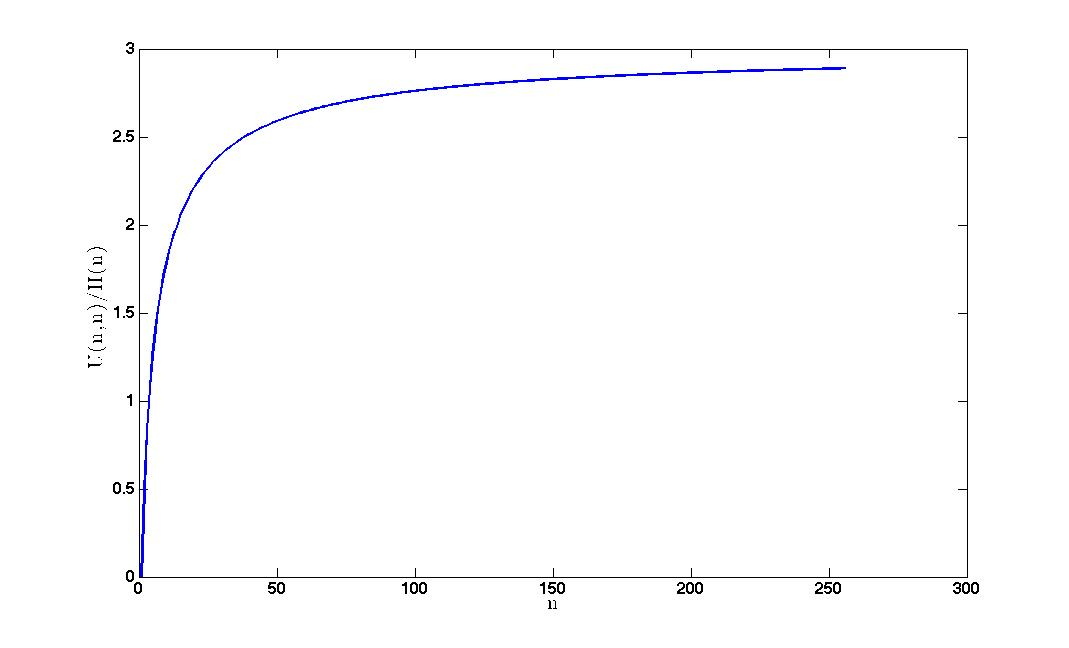
\includegraphics[width=0.8\textwidth]{fast_converge_plot.jpg} 
\caption{The approximation factor $U(n,n)/H(n)$ converges to the proposed upper
bound factor 3}
\label{fig:fast_converge_plot}
\end{figure}
\end{remark}


\paragraph{Better recursion equation:}
Let's rewrite the recursion equation as follows: 
\begin{equation} \label{eqn:cracking}
	U(t,n) = \min
\left\{
	\begin{array}{ll}
		\min_{\beta \in [1,n]} \bigg[U(t,n-\beta) + \frac{\beta}{n} \bound(n-\beta)
		\bigg]\\
		\rho_n U(t-1,n)
	\end{array}
\right.
\end{equation}
Indeed, we have two options: iterate on $n$ samples once, or choosing the best
sub-set size. Using the new formulation, the time
complexity reduces from $n^2t^2$ to $n^2 t$. We uses the new formulation in the
rest of the paper. 
\paragraph{Optimality of the heuristic procedure in large-scale learning:}
The next two lemmas try to justify our heuristic schedule for large-scale
learning, when $n \to \infty$.
\begin{lemma} \label{lemma:lowerbound_fast}
	For the fast convergence rate and $n\geq 10$, we have: 
	\begin{equation*}
		U(n,n) \geq \bound(n)
	\end{equation*}
\end{lemma}
\begin{proof}
	Let's do this by induction. If we compute the 
	value $U(10,10)$, we understand that $U(10,10)\geq \bound(10)$. 
	Assume $U(n,n)\geq \bound(n)$, according to equation \ref{eqn:cracking}, we
	have: 
	\begin{eqnarray*}
       &  \forall \beta \in \{1,\ldots,n-1\}\bigg[U(n,\beta) +
       \frac{n-\beta}{n} \bound(\beta) \bigg] \geq \bound(n) 
	\end{eqnarray*}
	For the fast convergence rate we have $\frac{n-\beta}{n} \bound(\beta) =
	\bound(\beta) -\bound(n)$. Therefore, the following inequality holds;
	\begin{equation}
		\forall \beta \in \{1,\ldots,n-1\}\bigg[U(n,\beta) +
        \bound(\beta) \bigg] \geq 2\bound(n) \label{eqn:lowerbound_n}
	\end{equation}
	Assume that $U(n+1,n)\geq (1-\frac{1}{n})\bound(n)$ holds; This gives us the
	following important inequality: 
	\begin{eqnarray}
       &  \forall \beta \in \{1,\ldots,n-1\}\bigg[U(n+1,\beta) +
       \bound(\beta) \bigg] \geq (2-\frac{1}{n})\bound(n) \label{eqn:n_plus}
	\end{eqnarray}
	 Using this we prove that $U(n+1,n+1)\geq
	\bound(n+1)$.
	To this end, we have to prove that:
	\begin{eqnarray}
       &  \forall \beta \in \{1,\ldots,n \}\bigg[U(n+1,\beta) +
        \bound(\beta) \bigg] \geq 2\bound(n+1) 
       \label{eqn:lowerbound_condition_1} \\
       & (1-\frac{1}{n+1}) U(n,n+1) \geq \bound(n+1) 
	\end{eqnarray}
	Let's start with the second inequality: 
	\begin{eqnarray}
       & (1-\frac{1}{n+1}) U(n,n+1) & \geq (1-\frac{1}{n+1}) U(n,n) \\
       & & \geq_{[U(n,n)\geq \bound(n)]} \frac{n}{n+1} \bound(n) \\
       & & = \bound(n+1)
	\end{eqnarray}
	Now, we prove the first inequality using inequality \ref{eqn:n_plus}: 
	\begin{eqnarray*}
       &  \forall \beta \in \{1,\ldots,n-1\}\bigg[U(n+1,\beta) +
       \bound(\beta) \bigg] \geq (2-\frac{1}{n})\bound(n) \geq 2 \bound(n+1)
	\end{eqnarray*}
	For $\beta = n$, we can use the assumption $U(n+1,n)\geq
	(1-\frac{1}{n})\bound(n)$ that yields us $U(n+1,n) + \bound(n)\geq 2
	\bound(n+1)$. It remains to proof $U(n+1,n) \geq (1-\frac{1}{n}) \bound(n)$; 
	If $U(n+1,n) = (1-\frac{1}{n})U(n,n)$, then obviously the inequality holds. 
	The challenging part is when 
	\[
	U(n+1,n) = \min_{\beta \in \{1,\ldots,n\}}  \bigg[ U(n+1,\beta) +H(\beta)
	\bigg] - \bound(n)
	\]
	Consider $\beta^* \in \{1,\ldots,n\}$ denotes to the minimizer of the above
	equation. So, we have
	\begin{eqnarray*}
		& U(n+1,n) & = U(n+1,\beta^*) + \bound(\beta^*) - \bound(n)\\
		& & = (1-\frac{1}{n}) U(n,\beta^*) +\bound(\beta^*) - \bound(n)\\ 
		& & = (1-\frac{1}{n})\bigg[ U(n,\beta^*) + \bound(\beta^*) \bigg] +
		\frac{1}{n} \bound(\beta^*)-\bound(n)\\ 
		& & \geq_{\text{Using \ref{eqn:lowerbound_n}} } 2 (1-\frac{1}{n}) \bound(n)
		+\frac{1}{n}  \bound(\beta^*) - \bound(n) \\ 
		& & \geq_{\beta^*\leq n-1}  2 (1-\frac{1}{n}) \bound(n) + \frac{1}{n-1}
		\bound(n) -\bound(n) \\ 
		& & = (1- \frac{1}{n} + \frac{1}{n-1}-\frac{1}{n})\bound(n) \geq
		(1-\frac{1}{n} )\bound(n)
	\end{eqnarray*}
	
\end{proof}
\begin{lemma}
	for all $n>5$, and fast convergence rate we have: 
	\begin{equation*}
		\frac{U(n+1,n+1)}{\bound(n+1)}\geq \frac{U(n,n)}{\bound(n)}
	\end{equation*}
\end{lemma}
\begin{proof}
	According to the equation \ref{eqn:cracking}, we have two possible formulations
	for $U(n+1,n+1)$. 
	\begin{itemize}
	  \item $U(n+1,n+1)= \rho_{n+1} U(n,n+1)$:
	  \begin{eqnarray*}
	  	& \frac{U(n+1,n+1)}{\bound(n+1)} & = \frac{\rho_{n+1} U(n,n+1)}{\bound(n+1)}
	  	\\ 
	  	& & \geq \frac{\rho_{n+1} U(n,n)}{\bound(n+1)} = \frac{\frac{n}{n+1}
	  	U(n,n)}{\bound(n+1)} \\
	  	& & = n U(n,n)  = \frac{U(n,n)}{\bound(n)}
	  \end{eqnarray*}
	  \item $U(n+1,n+1) = \min_{\beta \in \{ 1,\ldots,n \}} \left[
	  U(n+1,\beta) + \bound(\beta) \right] - \bound(n)$:
	    Consider the minimizer of the right side is $\beta^*$. There are two
	    possible values for $\beta^*$, $\beta^* \in \{ 1,\ldots,n-1\}$ or $\beta^*
	    = n$.
	    For the first case, we proceed as follows; 
	    \begin{eqnarray*}
	    	& U(n+1,n+1) & = 
	  U(n+1,\beta^*) + \bound(\beta^*) -\bound(n) \\ 
	  		& & = \rho_{\beta^*}U(n,\beta^*) + \bound(\beta^*) -\bound(n) \\ 
	  		& & = (1-1/\beta^*)U(n,\beta^*) + \bound(\beta^*) -\bound(n) \\ 
	  		& & = (1-1/\beta^*)\bigg[ U(n,\beta^*) + \bound(\beta^*) \bigg] +
	  		\frac{\bound(\beta^*)}{\beta^*} - \bound(n) \\ 
	  		& & \geq (1-1/\beta^*) U(n,n) + \frac{\bound(\beta^*)}{\beta^*} - \bound(n) 
	    \end{eqnarray*}
	    The last inequality is achieved by the assumption $\beta^* \in \{
	    1,\ldots,n-1\}$ and the recursion equation \ref{eqn:cracking}. Now, we try
	    to minimize the above respect to $\beta^*$: 
	    \begin{eqnarray*}
	    	& \min_{\beta^*} (1-1/\beta^*) U(n,n) + \frac{\bound(\beta^*)}{\beta^*} -
	    	\bound(n) \\ 
	    	& = U(n,n) - U(n,n)^2/4
	    \end{eqnarray*}
	    using the lower bound we can prove that $U(n+1,n+1)/\bound(n+1) \geq
	    U(n,n)/\bound(n)$: 
	    \begin{eqnarray*}
	    	& U(n+1,n+1)/\bound(n+1) & \geq \bigg[U(n,n) -
	    	U(n,n)^2/4\bigg]/\bound(n+1)
	    	\\ 
	    	& & = (n+1) \bigg[U(n,n) -
	    	U(n,n)^2/4\bigg]
	    \end{eqnarray*}
	    We have to prove this lower bound is greater than $U(n,n)/\bound(n)$. Here,
	    is just a few algebra: 
	    \begin{eqnarray*}
	    	& (n+1) \bigg[U(n,n) -
	    	U(n,n)^2/4\bigg] \geq n U(n,n) \\
	    	& \leftrightarrow U(n,n) - \frac{(n+1)}{4} U^2(n,n) \geq 0 \\ 
	    	& \leftrightarrow 1- \frac{(n+1)}{4} U(n,n) \geq 0 \\ 
	    	& \leftrightarrow 1\geq \frac{(n+1)}{4} U(n,n)
	    \end{eqnarray*}
	    We use the upper bound of $U(n,n) \leq 3 \bound(n)$ to prove that for
	    sufficient large $n$ the above inequality holds: 
	    \begin{equation*}
	    	\frac{(n+1)}{4} U(n,n) \leq \frac{3}{4}  (n+1)\bound(n) = \frac{3(n+1)}{4
	    	n} \leq 1 
	    \end{equation*}
	    The last inequality holds for all $n>5$. 
	\end{itemize}
\end{proof}
\begin{remark}
	Using above lemma we can prove that $U(n,n) = 3 \bound(n)$ when $n\rightarrow
	\infty$.
	From one hand, we know that $U(n,n) \leq 3 \bound(n)$. On the other hand, 
	$U(n,n)/\bound(n)$ is monotonically increasing respect to $n$ (as the above
	lemma says). The Figure \ref{fig:fast_converge_plot} confirms this asymptotical
	convergence.
\end{remark}
\paragraph{The condition number issue:}
So far, we assumed that $\frac{1}{m} \leq \frac{\mu}{L}$ for all $m<n$ and
consequently $\frac{\mu}{L}>\frac{1}{2}$. Now, we relax this assumption.
Obviously, using sample size $m<\frac{L}{\mu}$ wouldn't be reasonable. Before
that, Let's rewrite the convergence rate of SGD in this setting:
\begin{equation*}
	\risk_n(\wv^t) - \risk_n(\wv^*_n) \leq \frac{\kappa^2 v  }{t}, 
\end{equation*}
where we skip the parameter $v$ here. $\kappa = \frac{L}{\mu}$ is the condition
number. So, after one pass over data, i.e. $t = n$, we
will have:
\begin{equation*}
	\risk_n(\wv^n) - \risk_n(\wv^*_n) \leq \frac{\kappa^2 v d }{n} = \kappa^2 v
	\bound(n)
\end{equation*}
Now, our numerical computation of the recursion equation shows the
scheduling would be completely different. Assume $\kappa$ is an integer number. 
We want to prove that there is scheduling that can give us a better factor of
statistical precision for a single pass over data.The Case I. denotes to
generalization error of order $O(1/n)$ and Case II. denotes to the slow
convergence rate $O(1/\sqrt{n})$.
\begin{lemma}
	Assume $\epsilon_0 = 1$ and use the saga method then for all $m \geq \kappa$ \\
	\begin{itemize}
	  \item \textbf{Case I.}
	  \begin{eqnarray*}
		& U(2 m, m ) & \leq \frac{1}{2} (\frac{\kappa}{m})^2 + \bound(m)  \\ 
		& U(m,m) &  \leq \frac{2\kappa^2}{m^2} + 3 \bound(m)
	\end{eqnarray*}
	\item  \textbf{Case II.}
	  \begin{eqnarray*}
		& U(2 m, m ) & \leq \frac{1}{2}(\frac{\kappa}{m})^{1.4} + 0.6 \bound(m)
		\\
		& U(m,m) & \leq 2^{0.4} (\frac{\kappa}{m})^{1.4} + 1.6 \bound(m)
	\end{eqnarray*}
	\end{itemize}
\end{lemma}
\begin{proof}
    \textbf{Case I.} 
	For $m=\kappa$, we just iterate on the whole dataset: 
	\begin{equation*}
		U(2 \kappa, \kappa) \leq  (1-\kappa)^{2 \kappa} \epsilon_0 \leq \exp(-2) \leq
		\frac{1}{2} + \frac{1}{\kappa} 
	\end{equation*}
	Assume for $m$ the inequality holds, then we prove it holds for $m+1$ by
	induction: 
	\begin{eqnarray*}
		& U(2(m+1),m+1) & \leq (1-\frac{1}{m+1})^2 \bigg[ U(2m,m) + \frac{1}{m+1}
		\bound(m) \bigg] \\
		& & \leq \frac{m^2}{(m+1)^2} \bigg[ \frac{\kappa^2}{2 m^2} + \bound(m)
		+ \frac{1}{m+1} \bound(m) \bigg]
		\\
		& & = \frac{\kappa^2}{2 (m+1)^2} + \frac{m}{(m+1)^2} + \frac{m}{(m+1)^3} \\
		& & = \frac{\kappa^2}{2 (m+1)^2} + \frac{1}{m+1}- \frac{1}{(m+1)^2}+
		\frac{m}{(m+1)^3} \\ 
		& & = \frac{\kappa^2}{2 (m+1)^2} + \frac{1}{m+1} -\frac{1}{(m+1)^3} \\
		& & \leq \frac{\kappa^2}{2 (m+1)^2} + \frac{1}{m+1} = \frac{\kappa^2}{2
		(m+1)^2} + \bound(m+1)
	\end{eqnarray*}
	Now, we can devote all the budget on the half of samples to prove the second
	inequality: 
	\begin{eqnarray*}
		& U(m,m) & \leq U(m,\frac{m}{2}) + \frac{1}{2} \bound(\frac{m}{2}) \\ 
		& & \leq \frac{2\kappa^2}{m^2} + 3 \bound(m)
	\end{eqnarray*}
	\\
	\textbf{Case II.} 
	Assume for $m$ the inequality holds, then we prove it holds for $2m$ by
	induction: 
	\begin{eqnarray*}
		& U(4m,2m) & \leq (1-\frac{1}{2m})^{2m} \bigg[ U(2m,m) + \frac{1}{2}
		\bound(m) \bigg] \\
		& & \leq \exp(-1) \bigg[ \frac{\kappa^{1.4}}{2 m^{1.4}} 
		+ 1.1 \bound(m) \bigg]
		\\
		& & \leq  0.5 \frac{\kappa^{1.4}}{(2 m)^{1.4}} + 0.6 \bound(2m)
	\end{eqnarray*}
	If we devote all the budget on half of data set, then the latter
	inequality immediates.
\end{proof}
\begin{remark}
	Let's compare this results with SGD; After two passes over data, the
	convergence rate of SGD guarantees that $U(2n,n) \leq \frac{\kappa^2}{2}  \bound(n)$. While
	our proposed bound is $\frac{\kappa^2}{2n^2} + \bound(n)$. Since we have
	$\lim_{n\rightarrow \infty} \frac{\kappa^2}{2n^2\bound(n)} = 0$, our
	scheduling outperforms by factor $\kappa^2/2$ for considerably large $n$. 
\end{remark}
\begin{remark}
	The last Theorem breaks a wrong lower bound proposed at paper ``A Lower Bound
	for the Optimization of Finite Sums''. The paper suggests the lower bound $n+
	\sqrt{n(\kappa -1 )}\log(1/\epsilon)$ on number of required computation of
	stochastic gradient to obtain $\epsilon$ sub-optimality. For all $\epsilon>0$
	and $\kappa>1$, we need more than one pass over data. While we suggest
	suboptimality $\epsilon = \frac{2\kappa^2}{m^2} + 3 \bound(m)$ in just one pass
	over data. Please note this sub-optimality converge to zero for large $m$. So, definitly we can break this
	bound because of additional term $\sqrt{n(\kappa -1 )}\log(1/\epsilon)$ in the
	lower bound.
\end{remark}
\begin{remark}
	Let's compare the results with the recent paper ``Stop Wasting My Gradients:
	Practical SVRG''. In section 8, the authors suggest the time complexity 
	$(n+\kappa)d \log(\frac{1}{\epsilon})$ for SVRG. Consequently, they need
	$\log(n)$ passes over data to hit the generalization bound.
\end{remark}
\section{Appendix}
\paragraph{Analysis of Recursion Equation} 
We start with fast
convergence rate where $\bound(n) = 1/n$. In addition, we consider saga convergence rate for our
analysis means we assume $\rho_n = (1-\frac{1}{n})$. Now, we are equipped to
compute the optimal sample size increase: 
\begin{eqnarray*}
	& \arg \min_{\delta n} U_{\delta n}(t,n,\epsilon) & = \arg \min_{\delta
	n}\bigg[(1-\frac{1}{n+\delta n})\bigg(\epsilon + \frac{\delta n}{n+\delta n}
	\times \frac{1}{n}\bigg) + \frac{1}{n+\delta n}\bigg] \\
	& & = n \frac{1- \epsilon n}{1+\epsilon n } \bigg[= (\delta
	n)_{\min}\bigg]
\end{eqnarray*}

 Replacing this minimiser in equation \ref{eq:recursion_first}, give
us a simple quadratic equation respect to $\epsilon$:
\begin{equation}
	 \min_{\delta n} U_{\delta n}(t,n,\epsilon) = 
	-(\frac{n^2\epsilon^2  +(2 n- 4 n^2) \epsilon  - 4 n + 1}{4 n^2})
	\text{   [bound 1]}\label{eq:bound_1}
\end{equation}
Now, we have to compare this with one iteration on sample size $n$ means: 
\begin{equation*}
	U \left(t-1,n, \epsilon \rho_n \right) = \epsilon(1-\frac{1}{n}) + \frac{1}{n}
	\text{   [bound 2]} \label{eq:bound_2}
\end{equation*}
If we compare this bound with bound 1 (equation \ref{eq:bound_1}), we understand
that ([bound 1] - [bound 2]) is a quadratic equation respect to $\epsilon$ which
has a zero at $\epsilon = 1/n$ and is negative for all $\epsilon <
1/n$.
In other words, when the empirical sub-optimality on
$n$ sample is less than $1/n$ we can switch to the $n + \delta n$ samples.
As a simple example, when $\epsilon = 0.5/n$, then $\delta n = n/3$. For
different values of $\epsilon$ we will have different associated increase in
sample size $\delta n$. Therefore, one would come up with this question: it
is better to decrease the $\epsilon$ more or switch to the smaller $\delta n$.
What I want to conclude is that our trade-off is not precious using these
recursion equations. The function $U_{\delta n}$ is represented at Figure
\ref{fig:delta_n_plot} for different value of $\delta n$ when the $n = 1000$ and $\epsilon = 1/2000$. As the plot demonstrates the optimal $\delta n$ is $1000/3$ which matches to our analysis.
\begin{figure}
\center
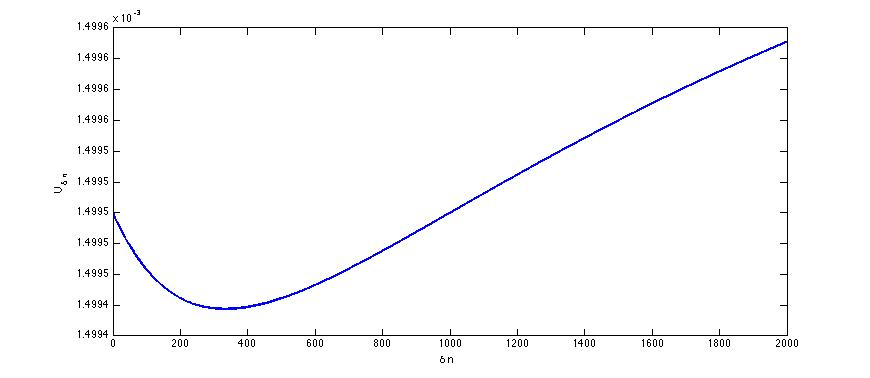
\includegraphics[width=0.8\textwidth]{optimal_delta.jpg} 
\caption{$U_{\delta n}$ VS $\delta n$}
\label{fig:delta_n_plot}
\end{figure}
According to our experiments after $2$ iterations on sample size $n$, the
recursion equations force us to increase the sample size by $1$ and iterate on
$n+1$ two times. This contradicts to our geometrical setting where we
showed if we are limited to one pass over data this scheduling is not optimal.
Please note in our geometrical setting, we formulate problem differently.
There, we fixed a constant step size $\delta n = n$ and we estimate a good step $t$, equivalently the sub-optimality $\epsilon$, for switching from
$n$ to $2n$ samples.
Now, I want to investigate the our pervious sample increasing strategy based on
our new formulation; Consider the partial derivative respect to $\delta n$ is:
\begin{equation*}
	\frac{\partial U_{\delta n}}{\partial \delta n} = 
	\frac{\delta n - n + \epsilon n^2
	+ \epsilon n \delta n}{n(\delta n + n)^3}
\end{equation*}
As long as the
derivative is negative we can increase sample size. This yields us the following
constraint: 
\begin{equation*}
	\delta n + \epsilon n^2 + \epsilon n \delta n \leq n 
\end{equation*}
Here, it turns out that $\delta n = n$ imposes a positive derivative means
we can obtain a better change of sample size in such condition. However, if
$\epsilon \rightarrow 0$, then the choice $\delta n = n$ would be the best
choice.\\
% Hadi's ==========================
\end{document}